\section{Results}
\label{sec:results}

\subsection{Delaunay triangulation algorithm}
\label{sub:results:triangulation}

We tested the Bowyer-Watson and Lawson triangulation algorithms for randomly generated inputs of different size.
%This is done by recursively adding $n$ points to the initial triangulation.

For each input size, 100 independent trials were performed and then averaged.
In \figref{fig:triangulation-runtime} we can see the average time that was needed for inserting $n$ points.
We see that both algorithms have the same complexity, and even effectively the same runtime.
Within our measurements, Lawson was slightly slower than Bowyer-Watson.

%The result without PSLG boundary segments is shown in Figure \ref{fig:triangulation/runtime} and
%with the segments in Figure \ref{fig:result_runtimeSegments}.

We repeated the same experiments for a constrained triangulation problem.
In addition to the randomly generated vertices, we now added a PSLG that constrained the triangulation.
The results are shown in \figref{fig:triangulation-pslg-runtime}.
Again the difference between the methods is fairly small.

In both cases, the complexity is steeper than linear in a log-log scale.
This indicates a steeper behaviour than polynomial, meaning exponential.
Theoretically, these algorithms should run in $O(n)$ (see \secref{sub:bowyer_watson}), implying our implementation has a weak searching step somewhere.

\begin{figure}[t!]
    \centering
    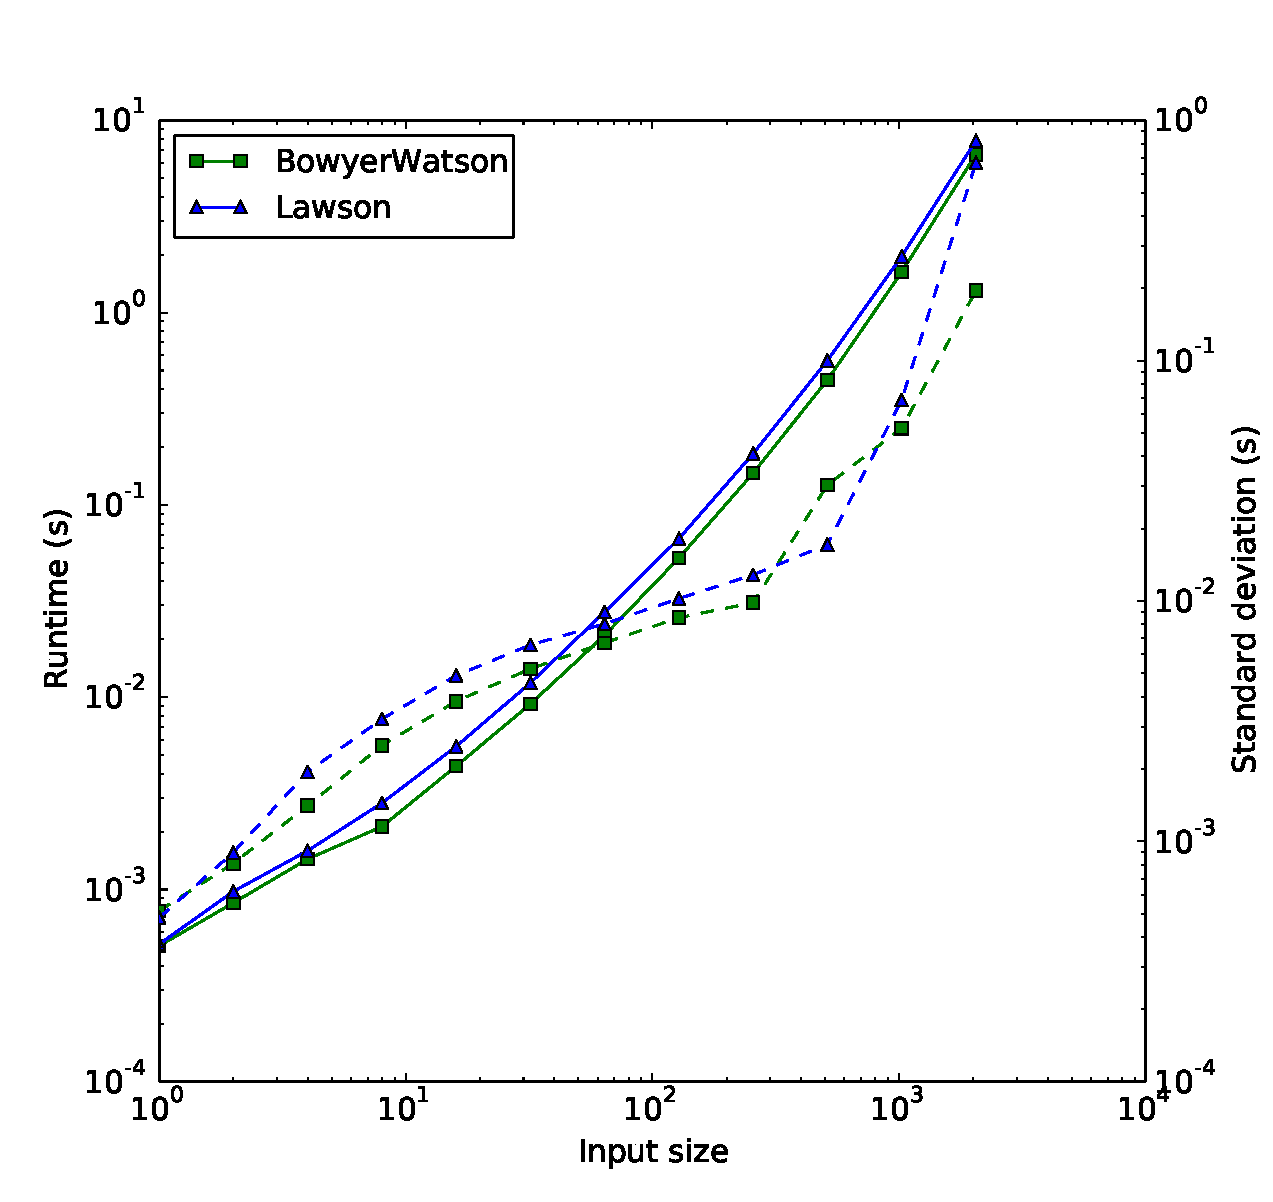
\includegraphics[width=\columnwidth]{../images/runtime.pdf}
    \label{fig:triangulation-runtime}
    \caption{Runtime for triangulation algorithms when input is unconstrained}
\end{figure}

\begin{figure}[t!]
    \centering
    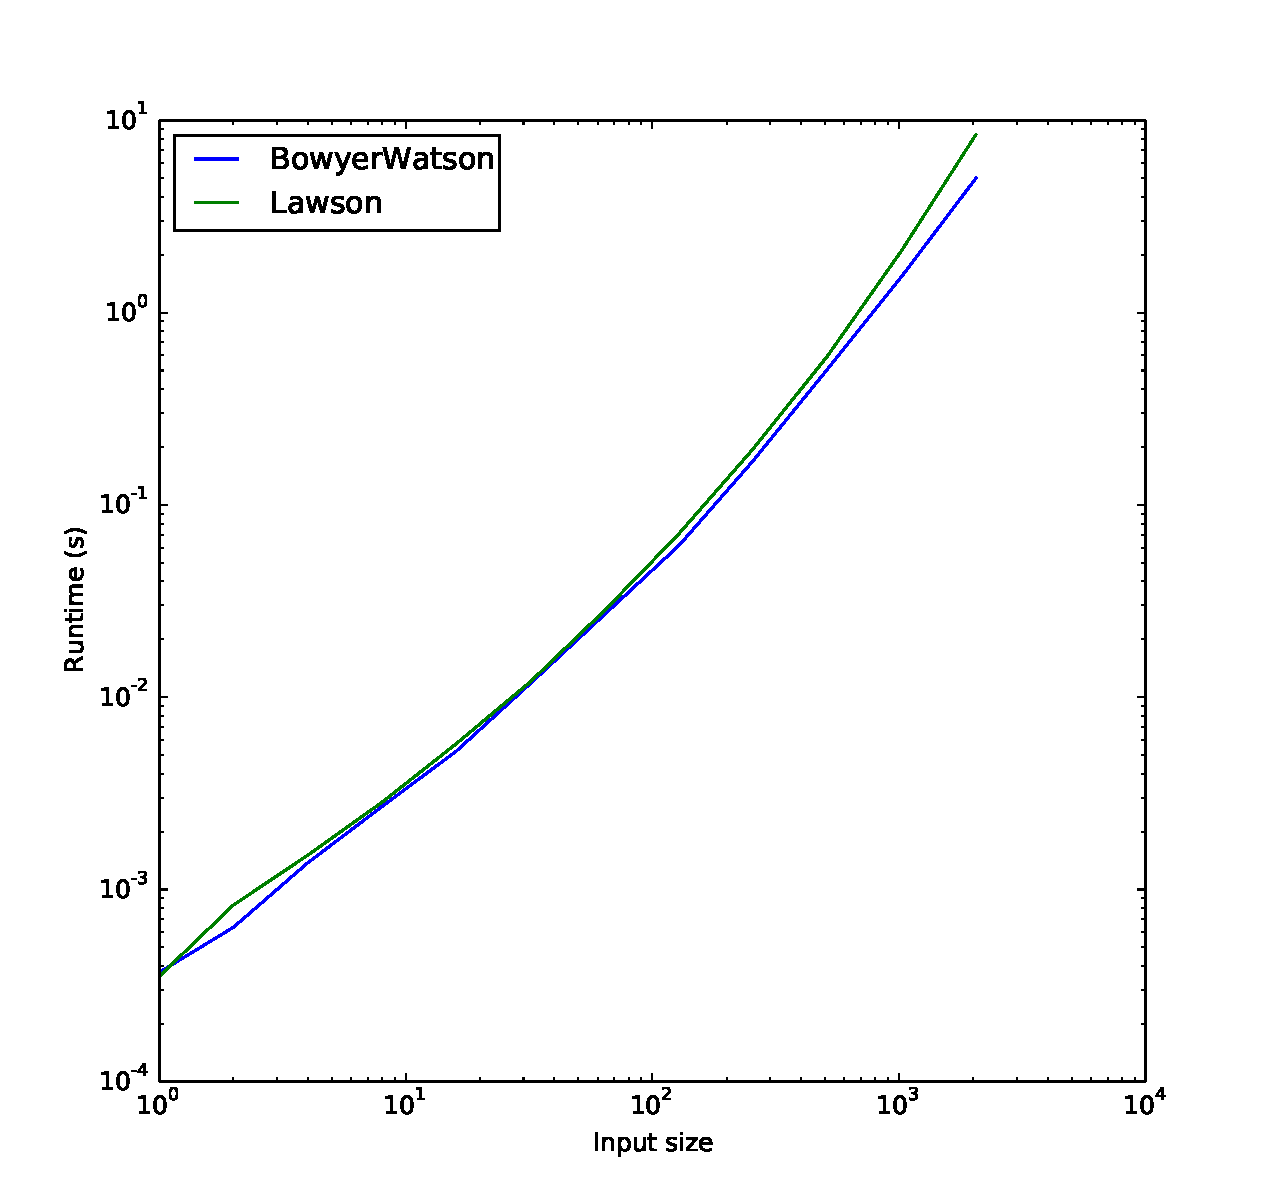
\includegraphics[width=\columnwidth]{../images/runtime_segments.pdf}
    \caption{Runtime for triangulation algorithms when input is constrained by a PSLG}
    \label{fig:triangulation-pslg-runtime}
\end{figure}

\subsection{Ruppert's refinement algorithm}
\label{sub:results:ruppert}

Ruppert's refinement algorithm has been used on a car-shaped case (see \figref{fig:result_Car20}) while two parameters of the algorithm were varied:
The maximum area of each triangle was restricted to values ranging from $50$ to $300$ and
the minimum angle within each triangle was restricted to values ranging from $10\degr$ to $30\degr$.
For the Delaunay triangulation we used Lawson's method, but Bowyer-Watson would give the same triangulation and complexity.
Unfortunately, the algorithm didn't converge for each setting, so the experiments were cut-off when they ran for more than $10$ seconds.

In \figref{fig:ruppert-runtime} the runtime as a function of the minimum angles is shown, while in \figref{fig:ruppert-runtime2} the runtime as a function of maximum area is shown.
In \figref{fig:ruppert-runtime}, the first thing to note is that, given a maximum area, there seems to be a convergence range in terms of minimum angle.
There seems to be a complex relationship with the maximum area concerning this conclusion since a `x00' area typically works for the lower angles, while a `x50' area works better for the higher angles.
The most-likely cause for this, is how easily triangles of a certain size may fit inside our domain: Ruppert's algorithm inserts points, but never removes points.
Thus, if it is off to a bad start, it may need unexpectedly many triangles near the boundary or not converge at all.

Generally, the best convergence is reached for an angle of around $20\degr-22.5\degr$.

\figref{fig:ruppert-runtime2} shows that as the maximum area decreases, the algorithm becomes exponentially slower.
This is easily explained by realising we need increasingly many triangles to fill the domain ($n$ increases), while
our implementation of the Delaunay triangulation algorithms scales exponentially with $n$.

% In \figref{fig:ruppert-runtime} we notice that the algorithm seems to converge fastest when we limit the smallest angle to about $23\degr$.
% When the angles are either big or small, the algorithm converges at a much slower rate.
% In \figref{fig:ruppert-runtime2} it can be seen that making the maximum area bigger generally makes the runtime slightly slower.
%Surprisingly, setups in which the maximum area is divisible by 100 seem to converge faster than other setups.
%Surprisingly we see that at certain minimum angles, the algorithm does converge when the maximum area is an even multitude of 50 ($0, 100, 200, \ldots$), but not when the maximum area is an uneven multitude of 50 ($50, 150, 250, \ldots$).

\begin{figure}[t!]
    \centering
    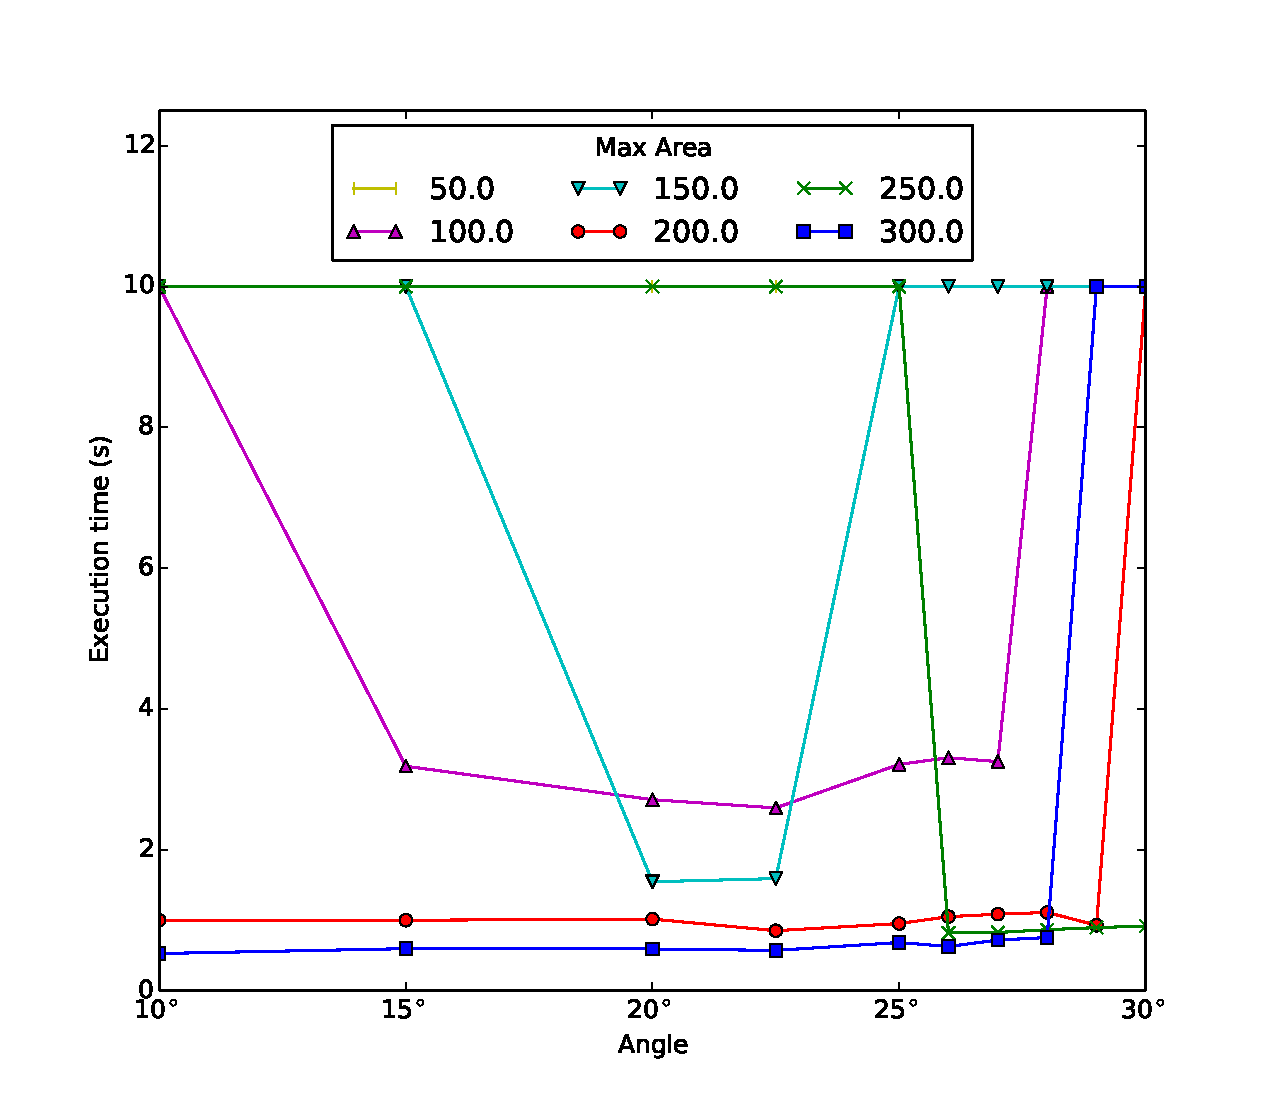
\includegraphics[width=\columnwidth]{../images/ruppert.pdf}
    \caption{Runtime of Ruppert's refinement algorithm for different angles. Note that an execution time of 10s means ``does not converge''.}
    \label{fig:ruppert-runtime}
\end{figure}

\begin{figure}[t!]
    \centering
    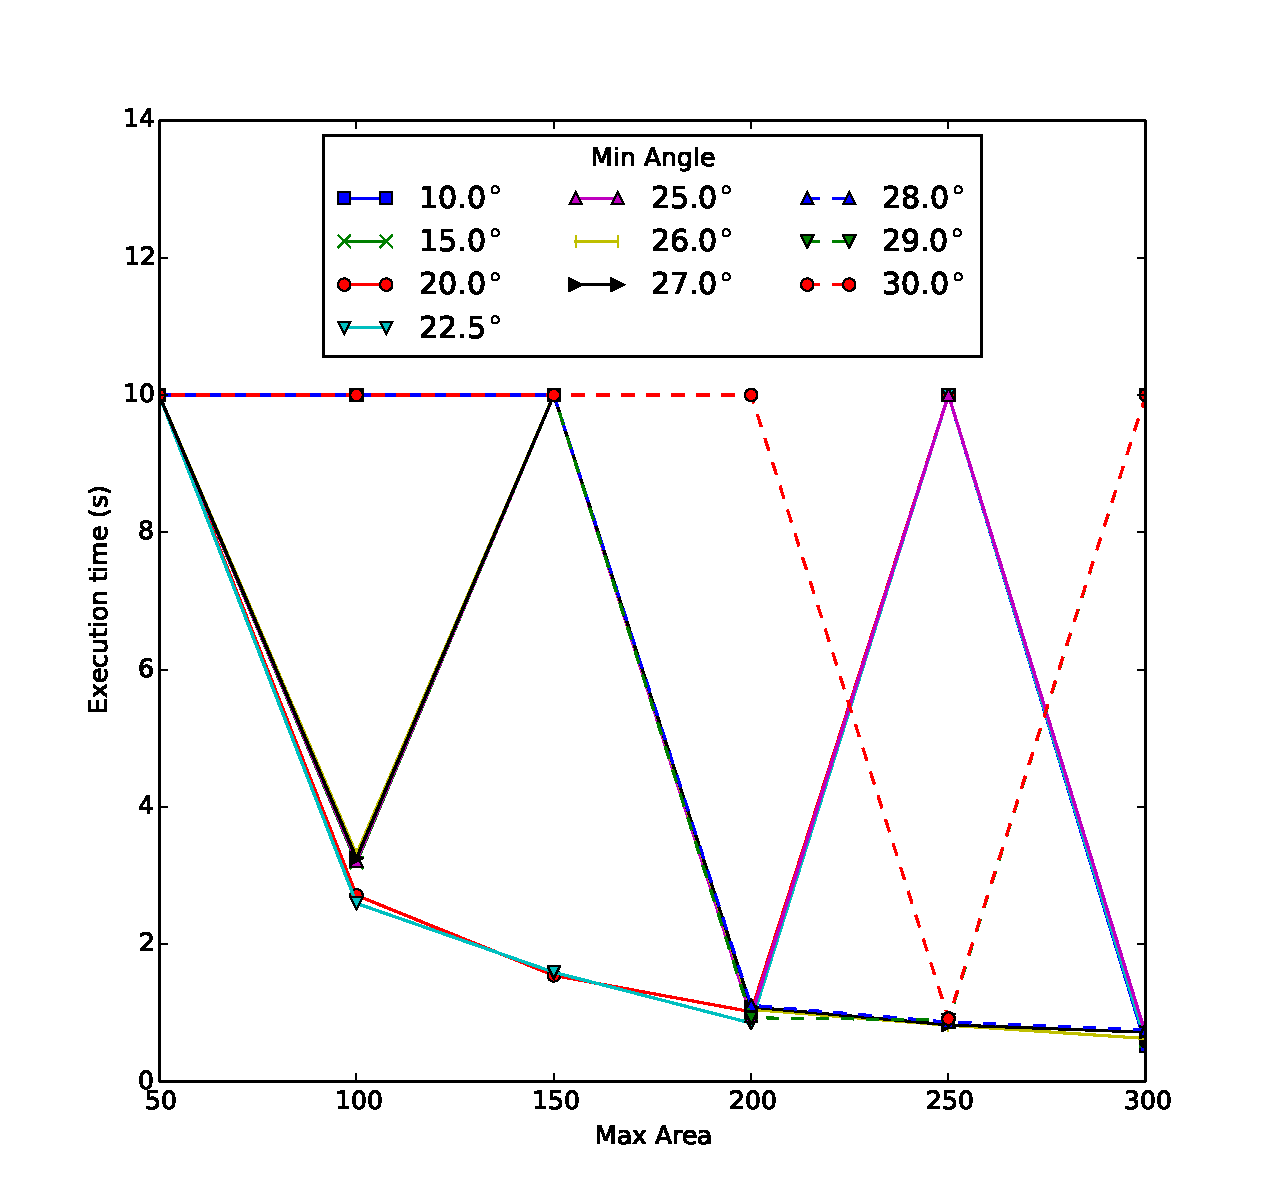
\includegraphics[width=\columnwidth]{../images/ruppert2.pdf}
    \caption{Like \figref{fig:ruppert-runtime}, but now as a function of the specified maximum cell area.}
    \label{fig:ruppert-runtime2}
\end{figure}

\begin{figure}
    \centering
    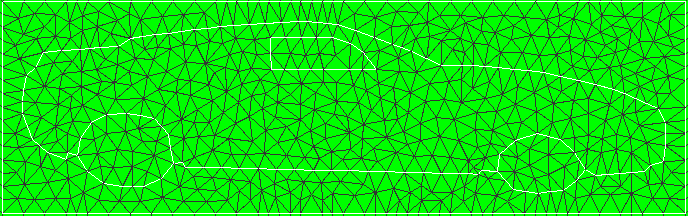
\includegraphics[width=\columnwidth]{../images/Car_Ruppert20.png}
    \caption{Triangulation generated using Ruppert's refinement algorithm for a car. The white lines are PSLG boundary elements.
    The criterea were set to a minimum angle of 20$\degr$ and a maximum area of 200.}
    \label{fig:result_Car20}
\end{figure}

\figref{fig:result_TU20} shows another triangulation generated using Ruppert's refinement algorithm.
We could not measure Ruppert's performance on this shape, because of a bug in our load function:
Our implementation of Lawson's and Bowyer-Watson's Delaunay algorithm, currently cannot load
boundary segments in an arbitrary order just yet.

\begin{figure}
    \centering
    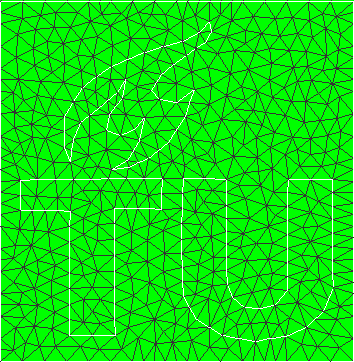
\includegraphics[width=\columnwidth]{../images/TU_Ruppert20.png}
    \caption{Triangulation generated using Ruppert's refinement algorithm for the TU Delft logo. The white lines are PSLG boundary elements.
    The criteria were set to a minimum angle of 20$\degr$ and a maximum area of 200.}
    \label{fig:result_TU20}
\end{figure}

Chew's second refinement algorithm has not been implemented successfully and thus no results are shown.


